\documentclass[pdf,notes]{beamer}
\mode<presentation>{\usetheme[secheader]{Boadilla}}

\usepackage{color,soul}
\usepackage{wrapfig}
\usepackage{mathtools}
\usepackage{xypic}
\usepackage[all,cmtip]{xy}
\usepackage{mystyle}
\includecomment{versiona}
\usepackage{xeCJK}
\usepackage{lpic}
\usefonttheme{professionalfonts}
\usepackage{etoolbox}

\newcommand{\red}[1]{{\color[rgb]{0.6,0,0}#1}}
\setbeamertemplate{theorems}[numbered] 

\usepackage{tikz}
\usetikzlibrary{shapes,arrows,patterns}
\renewcommand{\implies}{\Rightarrow}
\newcommand{\Sol}{\mathcal{S}\mbox{ol}}
\newcommand{\Ind}{\mbox{\normalfont Ind}}
\newcommand{\Hom}{\mbox{\normalfont Hom}}
\newcommand{\D}{\mathcal{D}}
\newcommand{\A}{\mathcal{A}}
\newcommand{\Co}{\mathbb{C}}
\newcommand{\X}{\mathbb{X}}
\renewcommand{\setminus}{\backslash}
\newcommand{\nin}{\not\in}
\newcommand{\tmop}[1]{\ensuremath{\operatorname{#1}}}
\newcommand{\tmtextbf}[1]{{\bfseries{#1}}}
\newcommand{\tmtextit}[1]{{\itshape{#1}}}
\newcommand{\mss}{//}
\newcommand{\mbb}{\backslash\backslash}
\newcommand{\mmm}{\mid\mid}
\catcode`\<=\active \def<{
\fontencoding{T1}\selectfont\symbol{60}\fontencoding{\encodingdefault}}
\catcode`\>=\active \def>{
\fontencoding{T1}\selectfont\symbol{62}\fontencoding{\encodingdefault}}
\newcommand{\assign}{:=}
\newcommand{\comma}{{,}}
\newcommand{\um}{-}
\newcommand{\sol}{\mathcal{S}ol(\R^{p,q};\lambda,\nu)}
\newcommand{\Op}{\mbox{\normalfont Op}}
\newcommand{\Res}{\operatorname{Res}\displaylimits}
\newcommand{\OpR}{\mbox{\it R}}

%%\makeatletter
%%\newenvironment<>{proofs}[1][\proofname]{\par\def\insertproofname{#1\@addpunct{.}}\usebeamertemplate{proof begin}#2}
%%{\usebeamertemplate{proof end}}
%%\makeatother

\newtheorem{prop}{命題}
\newtheorem{taggedpropx}{命題}
\newtheorem{remark}{注}
\newtheorem{cor}{系}
\newenvironment{taggedprop}[1]
 {\renewcommand\thetaggedpropx{#1}\taggedpropx}
  {\endtaggedpropx}

\AtBeginEnvironment{remark}{%
	    \setbeamercolor{block title}{bg=orange,fg=white}
		\setbeamercolor{block body}{bg=orange!20,fg=black}
}
\AtBeginEnvironment{fact}{%
	    \setbeamercolor{block title}{bg=green,fg=black}
		\setbeamercolor{block body}{bg=orange!20,fg=black}
}
\AtBeginEnvironment{cor}{%
	    \setbeamercolor{block title}{bg=blue,fg=white}
		\setbeamercolor{block body}{bg=orange!20,fg=black}
}

\setCJKmainfont[AutoFakeBold=true]{Hiragino Mincho Pro} %my Mac

\title[2つのゲーゲンバウアー多項式に\dots]{2つのゲーゲンバウアー多項式に関連する積分公式について\footnote{60 min talk}}

% A subtitle is optional and this may be deleted

\author[レオンチエフ・アレックス]{小林俊行\inst{1} \and \underline{レオンチエフ・アレックス}\inst{2}}

\institute[東大] % (optional, but mostly needed)
{
  \inst{1}%
  大学院数理科学研究科、カブリ数物連携宇宙研究機構\\
  東京大学
  \and
  \inst{2}%
  大学院数理科学研究科\\
  東京大学
  }

  \date[表現論とその周辺分野\dots]{RIMS共同研究(公開型)\\「表現論とその周辺分野の広がり」\\京都大学数理解析研究所}
% - Either use conference name or its abbreviation.
% - Not really informative to the audience, more for people (including
%   yourself) who are reading the slides online

\subject{表現論}

\begin{document}
\begin{frame}\titlepage\end{frame}

\begin{frame}{Outline}
	\tableofcontents
\end{frame}
\section{The Main Result}
\begin{frame}{Gegenbauer polynomials}
	Family of polynomials $\left\{ C_n^\alpha \right\}_{n=1}^{\infty}$ that form an orthogonal basis of $L^2\left( [-1,1],(1-x^2)^{\lambda-\frac{1}{2}}dx \right)$.\begin{equation*}
		\begin{array}[]{c}
			C_0^\lambda(x)=1;\\
			C_1^\lambda(x)=2\lambda x;\\
			C_2^\lambda(x)=-\lambda+2\lambda(1+\lambda)x^2;\\
			C_3^\lambda(x)=-2\lambda(1+\lambda)x+\frac{4}{3}\lambda(1+\lambda)(2+\lambda)x^3;\\
			C_4^\lambda(x)=\left(\frac{4+\lambda^3}{3}+4\lambda^2+\frac{8\lambda}{3}  \right)x^3+(-2\lambda^2-2\lambda)x.
		\end{array}
	\end{equation*}
	They also satisfy the second-order differential equation\begin{equation*}
		(1-x^2)y''-(2\lambda+1)xy'+n(n+\lambda)y=0.
	\end{equation*}
\end{frame}
\begin{frame}
	\begin{prop}\label{prop:exp-st-gg}
		\begin{equation}
			| s + t |^{2 \nu} = \sum_{\mbox{\scriptsize $\begin{array}[]{c}
			\ell, m = 0 \\ \ell + m : \tmop{even}
		\end{array}$}}^{\infty} a_{\lambda,\mu,\nu}^{\ell,m} C_\ell^{\lambda} (s) C_m^{\mu} (t),
			\label{eqn:exp-st-gg}
		\end{equation}
		{\scriptsize
		\begin{equation*}
	a_{\lambda,\mu,\nu}^{\ell,m}= \frac{ 2^{-2\nu}(\lambda + \ell) (\mu + m)  \Gamma (\lambda + \mu + 2 \nu + 1) \Gamma (\lambda)
  \Gamma (\mu)\Gamma \left( 2\nu +
1 \right)}{\Gamma \left( \lambda + \nu + \frac{\ell -
  m}{2} + 1 \right)  \Gamma \left( \mu + \nu -
  \frac{\ell - m}{2} + 1 \right) \Gamma \left( \lambda + \mu + \nu + \frac{\ell +
  m}{2} + 1 \right)\Gamma\left(  \nu+1-\frac{\ell+m}{2}\right)}
		\end{equation*}
	}
	\end{prop}
%%	Here, $C_{\ell}^\lambda(t)$ ($\lambda\in\mathbb{C},\ell\in\N$) is the Gegenbauer polynomial.
%%	\begin{remark}
%%		We could not find this formula in the literature.
%%	\end{remark}
\end{frame}
\note{TODO (speech):\begin{enumerate}
\item Do not use numbers like ``proposition 1'', ``proposition 3'' during the speech -- no one will remember them.
	Come up with some ``aliases'' (maybe, ``general proposition'', ``special case'' etc.).
	Or maybe, make one proposition to be theorem, another to be observation etc;
\end{enumerate}
}
%%\begin{frame}
%%	\begin{figure}[h]
%%		\centering
%%\begin{lpic}[]{wanted(0.75)}
%%	\lbl[bl]{3,15; \large$\begin{array}[]{c}
%%		\mbox{\it Expansion of $| s + t |^{2 \nu}$}\\\\\mbox{ in the form} \\\\
%%	| s + t |^{2 \nu} =	\\\\
%%	\sum_{\mbox{\scriptsize $\begin{array}[]{c}
%%\ell, m = 0 \\	 l + m\in2\N
%%\end{array}$}}^{\infty}
%%		a_{\lambda, \mu, \nu}^{\ell, m} C_{\ell}^{\lambda} (s) C_m^{\mu} (t)
%%	\end{array}$} %dot 
%%		
%%	\end{lpic}
%%		\label{fig:wanted}
%%	\vspace{-0.5cm}
%%	\caption*{Can we find the {closed expression} for $a_{\lambda,\mu,\nu}^{\ell,m}$ \underline{in literature}???}
%%	\end{figure}
%%\end{frame}
\begin{frame}
	In fact, we can do more:
	\begin{prop}\label{prop:exp-stz-gg}
		  \label{thm:4}For $\tmop{Re} \lambda, \tmop{Re} \mu > - \frac{1}{2}$,
		    $\tmop{Re} (\nu) > 0$ and $-1 \leqslant z \leqslant 1$ the following holds:
		      \begin{eqnarray}
			          & | s + t z |^{2 \nu}  = \sum_{l,
					  m = 0 \mid l + m\mbox{\scriptsize :even}}^{\infty} a_{l, m}
					          (z) C_l^{\lambda} (s) C_m^{\mu} (t), &  \nonumber\\
						      & a_{l, m} (z) = \frac{\Gamma \left( \nu + \frac{1}{2} \right) \Gamma
						      (\lambda) \Gamma (\mu) (\lambda + l) z^m }{(1 + \nu)_{- \frac{l + m}{2}} \sqrt{\pi} \Gamma
										      (\mu + m) \Gamma \left( \lambda + \nu + \frac{l - m}{2} + 1 \right)}&\nonumber
										      \\&\times{}_2 F_1 \left( \begin{array}{c}
								        \frac{l + m}{2} - \nu, \frac{m - l}{2} - \nu - \lambda\\
									      \mu + m + 1
									          \end{array} ; z^2 \right). & 
										          \nonumber
											    \end{eqnarray}
										    \end{prop}
										    This generalizes Proposition \ref{prop:exp-st-gg}.
\end{frame}
\note{TODO (slides):\begin{enumerate}
	\item investigate why LHS in Prop. \ref{prop:exp-stz-gg} is non-analytic, while RHS is seemingly analytic
\end{enumerate}
TODO (speech):\begin{enumerate}
	\item keep in mind the formula\begin{equation*}
			{}_2F_1\left( \begin{array}[]{c}
				a,b\\c
			\end{array};1\right)=\frac{\Gamma(c-a-b)\Gamma(c)}{\Gamma(c-a)\Gamma(c-b)},\quad \Re(c-a-b)>0
		\end{equation*}
		during the talk;
\end{enumerate}}
\begin{frame}
	Proposition \ref{prop:exp-st-gg} is equivalent to the integral equality
	\begin{taggedprop}{$\;1'$}
		\label{prop:int-st-gg}
		\begin{equation*}
			\int_{- 1}^1 \int_{- 1}^1 | s - t |^{2 \nu} (1 - s^2)^{\lambda - \frac{1}{2}}
			(1 - t^2)^{\mu - \frac{1}{2}} C_l^{\lambda} (s) C_m^{\mu} (t) d s d t
		\end{equation*}
		{\scriptsize
		\begin{equation}
			=\frac{(- \nu)_{\frac{l + m}{2}} (- 1)^{\frac{l - m}{2}} \pi^{\frac{1}{2}} (2
			\lambda)_l (2 \mu)_m \Gamma \left( \lambda + \frac{1}{2} \right) \Gamma \left(
			\mu + \frac{1}{2} \right) \Gamma \left( \nu + \frac{1}{2} \right) \Gamma
		(\lambda + \mu + 2 \nu + 1)}{l!m! \Gamma \left( \lambda + \nu + \frac{l -
		m}{2} + 1 \right) \Gamma \left( \mu + \nu - \frac{l - m}{2} + 1 \right) \Gamma
		\left( \lambda + \mu + \nu + \frac{l + m}{2} + 1 \right)}
			\label{eqn:int-st-gg}
			\tag{1$'$}
		\end{equation}
		}
	\end{taggedprop}
	Here I refer to \ref{prop:int-st-gg}.
\end{frame}
\section{Special cases}
\begin{frame}
	Furthermore,
	Letting $\lambda,\mu\to\infty$ (while keeping $\mu/\lambda=w\in\mathbb{R}$) and using
	\vspace{-0.3cm}
	\begin{equation*}
			H_n (x) = n! \lim_{\lambda \rightarrow \infty} \lambda^{- \frac{n}{2}}
			C_n^{\lambda} \left( \frac{x}{\sqrt{\lambda}} \right)
	\vspace{-0.4cm}
	\end{equation*}
	in Proposition \ref{prop:exp-st-gg}, we arrive at:
	\begin{cor}\label{cor:int-xzy-hh}
		For $\nu\in\mathbb{C}$, $w\in\R$ the following holds:
		\begin{equation*}
			\begin{array}[]{c}
			\int_{- \infty}^{\infty} \int_{- \infty}^{\infty} | x - w y |^{2 \nu} e^{-
			x^2 - y^2} H_\ell (x) H_m (y) d x d y \\= (- \nu)_{\frac{\ell + m}{2}} (- 1)^{\frac{\ell
			- m}{2}} 2^{\ell + m} \pi^{\frac{1}{2}} \Gamma \left( \frac{1}{2} + \nu \right)
			(w^2 + 1)^{\nu - \frac{\ell + m}{2}} w^m .
			\end{array}
		\end{equation*}
	\end{cor}
	\begin{remark}
		The particular case $k=2$ of \underline{Mehta integral}
	\vspace{-0.3cm}
		\begin{equation*}
			\frac{1}{(2\pi)^{k/2}}\int_{\mathbb{R}^k}\myabs{\Delta(\mathbf{t})}^{2\gamma}\exp\left( -\myabs{\mathbf{t}}^2/2 \right)d\mathbf{t}=\prod_{j=1}^k\frac{\Gamma\left( 
			1+j\gamma\right)}{\Gamma(1+\gamma)},\Delta(t):=\prod_{i<j}(t_i-t_j)
	\vspace{-0.4cm}
		\end{equation*}
		follows from this (take $w=1,\ell=m=0$).
	\end{remark}
\end{frame}
\note{
	TODO (slides):\begin{enumerate}
		\item investigate why LHS in Cor. \ref{cor:int-xzy-hh} is non-analytic, while RHS is seemingly analytic
	\end{enumerate}
	TODO (speech):\begin{enumerate}
	\item 
\end{enumerate}
}
\begin{frame}[fragile]{Hierarchy}
\begin{tikzpicture}
%mypipes
%        File: intdep.tex
%     Created: 土  1 07 11:00 PM 2017 J
% Last Change: 土  1 07 11:00 PM 2017 J
%
\documentclass[a4paper,12pt]{article}
\usepackage{pdflscape}
\usepackage{prerex,mystyle}
\usepackage[left=4pt,right=4pt]{geometry}
\usepackage[default,scale=0.92]{opensans}
\usepackage{dot2texi}
\usepackage{tikz}
\usetikzlibrary{shapes,arrows}
\renewcommand{\seriesdefault}{sb}
\renewcommand{\ttfamily}{\fontfamily{cmtt}\fontseries{m}\selectfont}

\newtheorem{theorem}{Theorem}
\newtheorem{remark}[theorem]{Remark}
\newtheorem{fact}[theorem]{Fact}
\newtheorem{proposition}[theorem]{Proposition}
\newtheorem*{proposition*}{Proposition}
\newtheorem*{remark*}{Remark}



\begin{document}
%%\thispagestyle{empty}
%%\setcounter{diagheight}{50}
%%\begin{chart}\sf
%%	\grid
%%\text 10,50:{\Large Computer\\\Large Science}
%%\reqfullcourse 50,45:{1083}{Comput.\,Sci.\\Concepts}{TTh 10:00}
%%\reqhalfcourse 25,40:{1303}{Discrete\\Structures}{MWF 9:30}
%%\reqhalfcourse 30,30:{2813}{Computer\\Organiz.\,I}{MWF 8:30}
%%  \prereq 50,45,30,30:
%%  \prereq 25,40,30,30:
%%\reqhalfcourse 45,30:{2023}{Procedural\\Prog.\,Devel.}{MWF 2:30}
%%  \prereq 50,45,45,30:
%%\reqhalfcourse 65,30:{2513}{Informat.\\Systems}{TTh 1:00}
%%  \coreq 50,45,65,30:
%%\mini 10,26:{1083}
%%\reqhalfcourse 10,20:{2333}{Computab.\,\&\\Formal\,Lang.}{TTh 11:30}
%%  \prereq 25,40,10,20:
%%  \prereq 10,26,10,20:
%%\reqhalfcourse 45,20:{2013}{Software\\Engineer.\,I}{MWF 11:30}
%%  \prereq 45,30,45,20:
%%\halfcourse 55,20:{2685}{\texttt{C++}\\Program.}{no}
%%  \prereq 45,30,55,20:
%%\mini 21,16:{2013}
%%\reqhalfcourse 15,10:{3323}{Data\\Structures}{MWF 10:30}
%%  \prereq 25,40,15,10:
%%  \prereq 21,16,15,10:
%%\reqhalfcourse 25,10:{3813}{Comput.\\Organiz.\,II}{TTh 8:30}
%%  \prereq 30,30,25,10:
%%\reqhalfcourse 35,10:{3413}{Operating\\Systems\,I}{MWF 9:30}
%%  \prereq 30,30,35,10:
%%  \recomm 45,20,35,10:
%%\halfcourse 45,10:{3013}{Software\\Engineer.\,II}{MWF 11:30}
%%  \prereq 45,20,45,10:
%%\halfcourse 58,10:{3513}{Database\\Mngt.\,Sys.\,I}{MWF 8:30 pm}
%%  \prereq 65,30,58,10:
%%  \prereq 45,20,58,10:
%%\reqhalfcourse 70,10:{3503}{Sys.\,Anal.\\\&\,Design}{TTh 10:00}
%%  \prereq 65,30,70,10:
%%\end{chart}
%%
%%\begin{center}
%%\begin{minipage}{6.0in}
%%\begin{itemize}
%%\item
%%A solid arrow \solidarrow\  indicates a required prerequisite, 
%%a dotted arrow \dottedarrow\ 
%%indicates a corequisite (to be taken before or concurrently), and a
%%dashed arrow \dashedarrow\ indicates a recommended prerequisite.
%%Core courses are in \boldbox\ boxes; 
%%other courses (i.e.,~options or prerequisites)
%%are in \lightbox\ boxes.
%%\item Timetabling abbreviations: M, T, W, Th, F=Mon, Tue, Wed, Thur, Fri, resp.; eve=7:00--9:50 pm; no=not offered.
%%\end{itemize}
%%\end{minipage}
%%\end{center}
%%\newpage
\begin{landscape}
	\newgeometry{left=-5cm,top=4cm,bottom=0cm,right=0cm}
	\vspace*{5cm}
\begin{dot2tex}[mathmode,dot,scale=0.9]
  digraph G {
	  War10 -> S [label="k_2=0"];
	  DF85 -> S [label=" ",texlbl="$\kern-0cm\begin{array}[]{c}p=n,\\m=0\end{array}$"];
	  TV03 -> S [label=" ",texlbl="$\kern-1.5cm k_1=0$"];
	  War09 -> TV03;
	  //KL -> WS [color="blue",dir=both]
	  //Sp -> DS [color="blue",dir=both]
	  //WS -> DS [dir=both]
	  S -> Sp [label=" ", texlbl="$\begin{array}[]{c}
	  k=2,\\ \alpha=\beta
  \end{array}$"]
  KL -> Sp  [label=" ", texlbl="$\kern-8cm \begin{array}[]{l}\\\\\\\\\\\\A=B\end{array}$"]
	  War10 -> War10p [label=" ",texlbl="$\begin{array}[]{l}\alpha_1=\beta_1,\\\alpha_2=\beta_2,\\k_1=k_2\end{array}$"];
	  KL -> War10p[label=" ",texlbl="$\kern-2cm A+B=\nu+1$"];
	  TV03 -> TV03p [label=" ",texlbl="$\begin{array}[]{l}k_1=k_2,\\ \alpha_1=1,\\\alpha_2=\beta_2\end{array}$"];
	  KL -> TV03p [label=" ",texlbl="$\kern-3cm A=0$"];
	  DF85 -> DF85p [label=" ",texlbl="$\begin{array}[]{l}p=n=1,\\m=r=1,\\ \alpha=\beta\end{array}$"];
	  KL -> DF85p [label=" ",texlbl="$\kern-3cm\nu=2$"];
	  AAR -> S[label=" ",texlbl="$\begin{array}[]{l}\\\\\\\\\qquad\qquad\qquad j=k=0\end{array}$"];
	  AAR -> AARp [label=" ",texlbl="$\begin{array}[]{l}n=2,\\j=l=k=1,\\ \alpha=\beta\end{array}$"];
	  KL -> AARp [label=" ",texlbl="$\kern1cm\begin{array}[]{l}A=B+1\\\end{array}$"]

    KL [shape="box",label="{\mbox{[KL]}}:3"];
    S [shape="box",label="\mbox{[S]}:3"];
    War10 [shape="box",label="\mbox{\cite{warnaar2010sl3}}:4"];
    DF85 [shape="box",label="\mbox{\cite{dotsenko1985four}}:3"];
    TV03 [shape="box",label="\mbox{\cite{tarasov2003selberg}}:4"];
    War09 [shape="box",label="\mbox{\cite{warnaar2009selberg}}:2n+2"];
    War10p [shape="box",label="\mbox{\cite{warnaar2010sl3}'}:2"];
    //WS [shape="box",label="\mbox{[WS]}:3"]
    Sp  [shape="box",label="\mbox{[S]'}:2"]
    //DS  [shape="box",label="\mbox{[DS]}:3"]
    TV03p [shape="box",label="\mbox{\cite{tarasov2003selberg}'}:2"]
    DF85p [shape="box",label="\mbox{\cite{dotsenko1985four}'}:2"]
    AAR [shape="box",label="\mbox{\cite{andrews1999special}}:2"]
    AARp [shape="box",label="\mbox{\cite{andrews1999special}}':2"]
    }
\end{dot2tex}
\end{landscape}
\begin{landscape}
	\newgeometry{left=-3.7cm,top=4cm,bottom=0cm,right=0cm}
	\vspace*{5cm}
\begin{dot2tex}[mathmode,dot]//fdp
  digraph G {
	  {rank=same War10 DF85 TV03 KLg}
	  {rank=same KL S}
	  {rank=same TV03p War10pp Spp DF85pp}
	  War10 -> S [label="k_2=0"];
	  DF85 -> S [label=" ",texlbl="$\begin{array}[]{c}p=n,\\m=0\end{array}$"];
	  S -> Spp [label=" ", texlbl="$\begin{array}[]{c}k=2,\\\alpha=\beta\end{array}$"]
	  TV03 -> S [label=" ",texlbl="$k_1=0$"]
	  War10 -> War10pp [label=" ",texlbl="$\begin{array}[]{c}k_1=k_2=1,\\\alpha_1=\beta_1,\\\alpha_2=\beta_2\end{array}$"];
	  KL -> Spp  [label=" ", texlbl="$\begin{array}[]{c}\\\\A=B\end{array}$"]
	  KL -> War10pp[label=" ",texlbl="$\kern5emA+B=\nu+1$"];
	  TV03 -> TV03p [label=" ",texlbl="$\begin{array}[]{c}k_1=k_2,\\ \alpha_1=1,\\\alpha_2=\beta_2\end{array}$"];
	  KL -> TV03p [label=" ",texlbl="$\kern-1.5cm A=0$"];
	  DF85 -> DF85pp [label=" ",texlbl="$\begin{array}[]{c}m=n=1,\\ \alpha'=\beta',\\\alpha=\beta\end{array}$"];
	  KL -> DF85pp [label=" ",texlbl="$\nu=2$"];
	  KLg -> KL [label=" ",texlbl="$\begin{array}[]{c}z=1,\\l=m=0\end{array}$"];

    KLg [shape="box",label="{\mbox{[KLg]}}:3"];
    KL [shape="box",label="{\mbox{[KL]}}:3"];
    S [shape="box",label="\mbox{[S]}:3"];
    Spp [shape="box",label="\mbox{[S]''}:2"]
    War10 [shape="box",label="\mbox{\cite{warnaar2010sl3}}:4"];
    DF85 [shape="box",label="\mbox{\cite{dotsenko1985four}}:3"];
    TV03 [shape="box",label="\mbox{\cite{tarasov2003selberg}}:4"];
    War10pp [shape="box",label="\mbox{\cite{warnaar2010sl3}''}:2"];
    TV03p [shape="box",label="\mbox{\cite{tarasov2003selberg}'}:2"]
    DF85pp [shape="box",label="\mbox{\cite{dotsenko1985four}''}:2"]
    }
\end{dot2tex}
\end{landscape}
%%    a_1 -> a_2 -> a_3 -> a_4 -> a_1;
%%    a -> b [label="E=mc^2"];

Formulae above are as follows:\begin{equation*}
	\begin{array}[]{ll}
		\mbox{[KL]}:&\iint_{D_\pm}\myabs{u-v}^{-\nu}u^A(1-u)^Av^B(1-v)^B\;du\;dv=\cdots,\\
		\mbox{[S]}:&\int_{D_k}\Pi_{i=1}^kt_i^\alpha(1-t_i)^\beta\Delta^{2\gamma}(t)\;dt=\cdots,\\
		\mbox{\cite{warnaar2010sl3}}:&\int_{C_{\beta_1,\gamma}^{k_1,k_2}}\Pi_{i=1}^{k_1}t_i^{\alpha_1-1}(1-t_i)^{\beta_1}\Pi_{j=1}^{k_2}s_j^{\alpha_2}(1-s_j)^{\beta_2}
		\Delta^{2\gamma}(t)\Delta^{2\gamma}(s)\Delta^{-\gamma}(t,s)\;dt\;ds,\quad\beta_1+\beta_2=\gamma+1,\\
		\mbox{\cite{tarasov2003selberg}}:&\displaystyle\int_{C^{k_1,k_2}_{\gamma}}\prod_{i=1}^{k_1}t_i^{\alpha_1-1}\prod_{j=1}^{k_2}s_j^{\alpha_2-1}(1-s_j)^{\beta_2-1}\Delta^{2\gamma}(t)\Delta^{2\gamma}
		(s)\Delta^{-\gamma}(t,s)\;dt\;ds,\\
		\mbox{\cite{dotsenko1985four}}:&\displaystyle\int_{[0,1]^p}\int_{[1,\infty]^{n-p}}\int_{[0,1]^r}\int_{[1,\infty]^{m-r}}\prod_{i=1}^nt_i^\alpha(1-t_i)^\beta
		\prod_{j=1}^m\tau_j^{\alpha'}(1-\tau_j)^{\beta'}\Delta^{-2}(t,\tau)\Delta^{2\gamma}(t)\Delta^{2\gamma}(\tau)\;dt\;d\tau=\cdots,\\
		&{\alpha}/{\alpha'}={\beta}/{\beta'}=-\gamma,\quad\gamma\gamma'=1,\\
%%		\mbox{\cite{warnaar2010sl3}}':&\sin\mybra{\pi\beta_1}\iint_{D_-}u^{\alpha_1}(1-u)^{\beta_1}v^{\alpha_2}(1-v)^{\beta_2}\myabs{u-v}^{-\gamma}\;du\;dv+\\
%%		&+\sin\mybra{\pi\beta_2}\iint_{D_+}u^{\alpha_1}(1-u)^{\beta_1}v^{\alpha_2}(1-v)^{\beta_2}\myabs{u-v}^{-\gamma}\;du\;dv=\cdots,\quad \beta_1+\beta_2=\gamma+1,\\
%%		\mbox{[S]'}:&\iint_{D_-}\myabs{u-v}^{2\gamma}u^\alpha v^\alpha(1-u)^\beta(1-v)^\beta\;du\;dv,\\
		\mbox{[WS]}:&\;_3F_2\left(\begin{array}[]{c}
			a,1-a,c\\ d,2c-d+
		\end{array};1\right)=\cdots,\quad\mbox{a.k.a Whipple's sum},\\
		\mbox{[DS]}:&\;_3F_2\left(\begin{array}[]{c}
			a,b,c\\a-b+1,a-c+1
		\end{array};1\right)=\cdots,\quad\mbox{a.k.a Dixon's well-poised sum},\\
		\mbox{\cite{dotsenko1985four}'}:&\iint_D\myabs{u-v}^{-2}u^\alpha(1-u)^\beta v^{\alpha'}(1-v)^{\beta'}\;du\;dv,\quad \alpha/\beta=\alpha'/\beta',\\
		\mbox{\cite{andrews1999special}}:&\displaystyle\int_{[0,1]^n}\prod_{i=1}^jx_i\prod_{i=j+1}^{j+k}(1-x_i)\prod_{i=1}^kt_i^\alpha(1-t_i)^\beta\Delta^{2\gamma}(t)\;dt=\cdots,
	\end{array}
\end{equation*}

Above and below the following notations are used:\begin{equation*}
		\begin{array}[]{c}
			D_n:=\left\{ (t_i)_{i=1}^{n}\in\R^n\mid0\le t_1\le t_2\le\dots\le t_n\le1 \right\},\\
			D:=[0,1]^2,\\
			D_{\pm}:=\mysetn{\left( u,v \right)\in D}{(\pm)(u-v)>0},\\
			\displaystyle\Delta^\lambda\left( \left\{ x_i \right\}_{i=1}^n \right):=\prod_{1\le i<j\le n}\myabs{x_i-x_j}^{\lambda},\\
			\displaystyle\Delta^\lambda\left( \left\{ x_i \right\}_{i=1}^m,\left\{ y_j \right\}_{j=1}^n \right):=\prod_{i,j=1}^{m,n}\myabs{x_i-y_j}^\lambda.
		\end{array}
	\end{equation*}
	Moreover:\begin{itemize}
		\item the $\dots$ denotes the product ratio of product of Gamma functions;
		\item blue arrows imply the use of the proposition below;
	\end{itemize}
\begin{proposition*}
	\begin{equation*}
		\begin{array}[]{c}
			\iint_{D_-}u^{A_+}(1-u)^{A_-}v^{B_+}(1-v)^{B_-}\myabs{u-v}^{-\gamma}\;du\;dv=\dots\;_3F_2\left( \begin{array}[]{c}
				-A_-,A_++1,A_++B_+-\gamma+2\\
				B_-+A_++B_+-\gamma+3,A_+-\gamma+2
			\end{array};1\right)
		\end{array}
	\end{equation*}
\end{proposition*}
The literature read by me so far and referenced above is as follows:
\small
\nocite{*}
\bibliography{intdep}
\bibliographystyle{alpha}
\end{document}

\end{tikzpicture}
\end{frame}
\newcommand{\mypgf}{{\mbox{\bf product of Gamma functions}}}
\begin{frame}[fragile]
	\scriptsize
    \setul{0.5ex}{0.3ex}
	\definecolor{Blue}{rgb}{0,0.0,1}
	\definecolor{Red}{rgb}{1,0.0,0}
    \setulcolor{Blue}
	\ul{Selberg'44}
	\begin{wrapfigure}{r}{0.6\textwidth}
		\vspace{-30pt}
		  \begin{center}
			  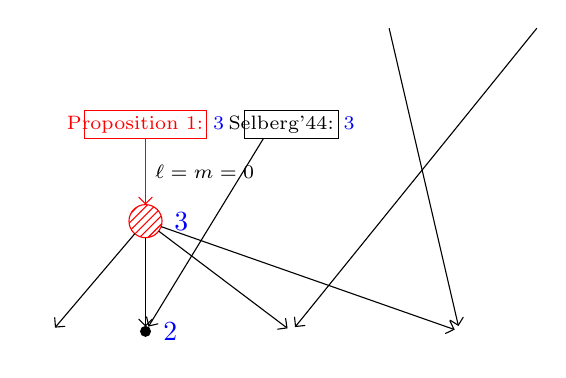
\begin{tikzpicture}[scale=0.7]
				\draw[color=red] (2.1,-2.0) rectangle (4.3,-2.5);
\node at (3.2,-2.25) {\color{red}{\scriptsize Proposition 1: \color{blue}{3}}};
\draw[color=black] (5.0,-2.0) rectangle (6.7,-2.5);
\node at (5.85,-2.25) {\color{black}{\scriptsize Selberg'44: \color{blue}{3}}};
\filldraw[color=red,pattern color=red,pattern=north east lines] (3.2,-4.0) circle(0.3);
\node at (3.85,-4.0) {\color{blue}{3}};
\fill[color=black] (3.2,-6.0) circle(0.1);
\node at (3.6500000000000004,-6.0) {\color{blue}{2}};
\draw[->,>=angle 90,color=red] (3.2,-2.5) -- node {\color{black}{\scriptsize $\kern1.5cm\ell=m=0$}} (3.2000000000000006,-3.7) ;
\draw[->,>=angle 90,color=black] (3.0057054739713385,-4.2285817953278375) -- node {} (1.5573628100792203,-5.93251434108327) ;
\draw[->,>=angle 90,color=black] (3.2,-4.3) -- node {} (3.2,-5.914999999999999) ;
\draw[->,>=angle 90,color=black] (3.4394567450999696,-4.180722071773562) -- node {} (5.777393604812446,-5.9452027206131675) ;
\draw[->,>=angle 90,color=black] (3.4830799946398643,-4.099326313908724) -- node {} (8.810326217188193,-5.968535514802874) ;
\draw[->,>=angle 90,color=black] (5.34,-2.5) -- node {} (3.252164719493017,-5.914683869988056) ;
\draw[->,>=angle 90,color=black] (10.3,-0.5) -- node {} (5.912899489957162,-5.922259057356316) ;
\draw[->,>=angle 90,color=black] (7.62,-0.5) -- node {} (8.877333022939228,-5.902602832941987) ;

				\end{tikzpicture}
			        \end{center}
				%\caption{A gull}
		\vspace{-60pt}
	  \end{wrapfigure}
	 \begin{equation*}
		\begin{array}[]{c}
		\displaystyle\int_{t \in [0, 1]^k} \displaystyle\prod\displaylimits_{i=1}^k t_i^{\alpha-1}(1-t_i)^{\beta-1} \displaystyle\prod\displaylimits_{1\le i<j\le k}\myabs{t_i-t_j}^{2\gamma} d
				t\\=\mypgf,\\
				\tmop{Re} (\alpha), \tmop{Re} (\beta) > 0, | \gamma | \ll 1
		\end{array}
			\end{equation*}
			\xymatrix{\ar[dddr]^{\begin{array}[]{c}
			k=2,\\ \alpha=\beta
		\end{array}}\\\\\\\;&}
		\vspace{-60pt}
		\begin{flushright}
    			\setulcolor{Red}
			\ul{Proposition 3}
		\end{flushright}
		\begin{flushright}
			\hspace{0.5\textwidth}\xymatrix{&\ar[ld]^{\begin{array}[]{c}
				\ell=m=0,\\ \lambda=\mu
		\end{array}}\\\\&}
		\end{flushright}
		\vspace{-40pt}
			\begin{equation*}
				\begin{array}[]{c}
				\displaystyle\iint_{[0, 1]^2} s^{\alpha-1}t^{\alpha-1}(1-t)^{\alpha-1}(1-s)^{\alpha-1} \myabs{s-t}^{2\gamma} dsdt
				\\=\mypgf
				\end{array}
			\end{equation*}
%%	\end{description}
\end{frame}
\begin{frame}{Hierarchy (Warnaar'10)}
	\scriptsize
	\fbox{Warnaar'10} is the generalization of Selberg integral shown in \cite[(1.4)]{warnaar2010sl3}\begin{equation*}
			\begin{array}{c}
				  \displaystyle\int_{(s, t) \in C_{\beta_1, \gamma}^{k_1, k_2} [0, 1]} \Pi^{\alpha_1 - 1,
					    \beta_1 - 1} (t) \Pi^{\alpha_2 - 1, \beta_2 - 1} (s) \Delta^{2 \gamma} (t)
					      \Delta^{2 \gamma} (s) \Delta^{- \gamma} (t, s) d s d t\\
					        = \mypgf,\\
					  \mbox{where }\beta_1 + \beta_2 = \gamma + 1,\\
					    \tmop{Re} (\alpha_i), \tmop{Re} (\beta_i) > 0,  \myabs{\gamma} \ll 1 ; \quad 1
						\le \forall i \le \displaystyle\min_i \{ k_i \} : \beta_1 + (i - k_2 - 1)
						  \gamma \nin \mathbb{Z}
			\end{array}
			\end{equation*}
			$\Delta^{-\gamma}(t,s):=\prod_{i,j=1}^{k_1,k_2}\myabs{t_i-s_j}^{-\gamma}$ and $C^{k_1,k_2}_{\beta_1,\gamma}[0,1]$ is some {\it linear sum} of subsets of $[0,1]^{k_1+k_2}$.
			Its particular case $k_1=k_2=1,\alpha_1=\beta_1,\alpha_2=\beta_2$ with LHS being\begin{equation*}
				\left(\displaystyle\iint\displaylimits_{\begin{array}[]{c}
					[0,1]^2\\t<s
				\end{array}}+\frac{\sin(\pi\alpha_1)}{\sin(\pi\alpha_2)}\displaystyle\iint\displaylimits_{\begin{array}[]{c}
					[0,1]^2\\t>s
			\end{array}} \right)(t(1-t))^{\alpha_1 - 1}  (s(1-s))^{\alpha_2 - 1}  | t - s |^{- \gamma} d s d t
			\end{equation*}
			is generalized by Proposition \ref{prop:int-st-gg}.
\end{frame}
\begin{frame}{Hierarchy (Tarasov-Varchenko'03)}
	\scriptsize
	\fbox{Tarasov-Varchenko'03} is another generalization of Selberg integral shown in \cite[(3.4)]{tarasov2003selberg}\begin{equation*}
\begin{array}{c}
  \displaystyle\int_{(s, t) \in C_{\gamma}^{k_1, k_2}} \Pi^{\alpha - 1, \beta_1 - 1} (t)
  \Pi^{0, \beta_2 - 1} (s) \Delta^{2 \gamma} (t) \Delta^{2 \gamma} (s)
  \Delta^{- \gamma} (t, s) d s d t \\
  =\mypgf,\\
  \mbox{where }\tmop{Re} (\alpha_i), \tmop{Re} (\beta_2) > 0, | \tmop{Re} \gamma | \ll 1
\end{array}
			\end{equation*}
			and $C^{k_1,k_2}_\gamma[0,1]$ is some another {\it linear sum} of subsets of $[0,1]^{k_1+k_2}$.
			Its particular case $k_1=k_2,\beta_2=1,\alpha=\beta_1$ with LHS being\begin{equation*}
				\displaystyle\iint\displaylimits_{\begin{array}[]{c}
				(s, t) \in [0, 1]^2\\t<s
			\end{array}} s^{\alpha - 1} (1 - s)^{\alpha - 1} \myabs{s-t}^{- \gamma} d s d t
			\end{equation*}
			is generalized by Proposition \ref{prop:int-st-gg}.
\end{frame}
\begin{frame}{Hierarchy (Dotsenko-Fateev'85)}
	\scriptsize
	\fbox{Dotsenko-Fateev'85} is yet another generalization of Selberg integral shown in \cite[(A35)]{dotsenko1985four}\begin{equation*}
\begin{array}{c}
  \frac{1}{n!m!} \int_{(t, \tau) \in [0, 1]^{n + m}} \Pi^{\alpha', \beta'} (t)
  \Pi^{\alpha, \beta} (\tau) \Delta^{2 \rho'} (t) \Delta^{2 \rho} (\tau)
  \Delta^{- 2} (t, \tau) d \tmop{td} \tau \\
  =\mypgf,\\
  \alpha' = - \rho' \alpha, \beta' = - \rho' \beta, \rho' \rho = 1,\\
  \tmop{Re} (\rho) < 0, \quad \tmop{Re} (\alpha), \tmop{Re} (\beta) > (n - 1)
  + | \tmop{Re} (\rho) | (m - 1)
\end{array}
			\end{equation*}
			Its particular case $m=n=1,\alpha'=\beta',\alpha=\beta$ with LHS being\begin{equation*}
				\displaystyle\iint\displaylimits_{(t, \tau) \in [0, 1]^2} t^{\alpha'} (1 - t)^{\alpha'} \tau^{\alpha} (1
				- \tau)^{\alpha} | t - \tau |^{- 2} d \tmop{td} \tau
			\end{equation*}
			is generalized by Proposition \ref{prop:int-st-gg}.
\end{frame}
\begin{frame}
	Furthermore, making variable change $w=s-t$ in Corollary \ref{cor:int-xzy-hh} and taking $z=1$ we arrive at\footnote[frame]{FIXME: check correctness}:
	\begin{cor}
		The following holds:
		\begin{equation}
			\mathcal{M}(hr_n\ast hr_m)(s)=
			\left(  \frac{1-s}{2}\right)_{\frac{l + m}{2}} (- 1)^{\frac{l
			+ m}{2}}  \pi^{\frac{1}{2}} \Gamma \left( \frac{s}{2} \right)
			2^{\frac{s-3}{2} + \frac{l + m}{2}}.
%%			\begin{array}[]{c}
%%			\int_{- \infty}^{\infty} \int_{- \infty}^{\infty} | x - y |^{2 \nu} e^{-
%%			x^2 - y^2} H_l (x) H_m (y) d x d y \\= (- \nu)_{\frac{l + m}{2}} (- 1)^{\frac{l
%%			- m}{2}} 2^{l + m} \pi^{\frac{1}{2}} \Gamma \left( \frac{1}{2} + \nu \right)
%%			2^{\nu - \frac{l + m}{2}} .
%%			\end{array}
			\label{eqn:mellin-hh}
		\end{equation}
	\end{cor}
	where $\mathcal{M}(\cdot)$ is the Mellin transform\begin{equation*}
		\left\{ \mathcal{M}(f) \right\}(s)=\int_0^\infty x^{s-1}f(x)\;dx,
	\end{equation*}
	and $hr_n$ are \underline{Hermite-Rodriguez} functions \cite{335863}
	\begin{equation*}
		hr_n(x):=H_n(x)e^{-x^2}.
	\end{equation*}
	Applying inverse Mellin transform, we arrive at the well-known formula for convolution of Hermite-Rodriguez functions.
\end{frame}
\note{TODO (slides):\begin{enumerate}
\item make the Corollary better;
\item Fock表現のK-typeの具体的表示に関連して、セミナー中にかなり丁寧に説明しました。
\end{enumerate}}
\section{Proof}
\begin{frame}{Method 1 (direct) (1/2)}
	\scriptsize
	We show Proposition \ref{prop:int-st-gg} as:
	\begin{enumerate}
		\item Using the property $
				(1-x^2)^{\alpha-\frac{1}{2}}C_n^\alpha(x)=a(\alpha,n)
				\frac{d^n}{dx^n} (1-x^2)^{n+\alpha-\frac{1}{2}}, a(\alpha,n):=\frac{(-1)^n}{2^nn!}\frac{\Gamma\left( \alpha+\frac{1}{2} \right)\Gamma\left( n+2\alpha \right)}{\Gamma(2\alpha)\Gamma\left(\alpha+n+\frac{1}{2}  \right)}$
				of Gegenbauer polynomials and integration by parts we have ${\mbox{LHS}\eqref{eqn:int-st-gg}}/{a(\lambda,l)/a(\mu,m)}=$\begin{equation}
					\kern-1.2cm
					\iint\displaylimits_{[-1,1]^2}
					\kern-0.2cm| s - t |^{2 \nu} \frac{\partial^l}{\partial s^l}(1-s^2)^{\lambda+l-\frac{1}{2}}\frac{\partial^m}{\partial t^m}(1-t^2)^{\mu+m-\frac{1}{2}}
					\kern-0.1cm=(-1)^m(-2\nu)_{l+m}\kern-0.2cm\iint\displaylimits_{[-1,1]^2}\kern-0.2cm\myabs{s-t}^{2\nu-l-m}(1-s^2)^{\lambda+l-\frac{1}{2}}(1-t^2)^{\mu+m-\frac{1}{2}};
					\label{eqn:m1-1}
				\end{equation}
			\item Upon change of variables $s=(1-t)(1-w)+t$ and using Euler's integral representation 
					\vspace{-0.2cm}
				\begin{equation*}
					B(b,c-b){}_2F_1(\begin{array}[]{c}
						a,b\\c
					\end{array};z)=\textstyle\int_0^1x^{b-1}(1-x)^{c-b-1}(1-zx)^{-a}dx,\quad\Re(c)>\Re(b)>0
					\vspace{-0.2cm}
				\end{equation*}
				of ${}_2F_1$
			we have ${\mbox{RHS}\eqref{eqn:m1-1}}/{(-1)^m/(-2\nu)_{l+m}}/2^{\lambda+l-\frac{1}{2}} =$
			\vspace{-0.2cm}
			\begin{equation}
				\kern-1.2cm
				B \left( 2\nu-l-m+1, \lambda+l-\frac{1}{2} \right)
				\kern-0.2cm\int_{-1}^1 (1 - t)^{2 \nu+\lambda-m+\frac{3}{2}} {}_2 F_1 \left( \kern-0.2cm\begin{array}{c}
					\frac{1}{2}-l-\lambda, 2\nu-l-m+1\\
					2 \nu+\lambda-m+\frac{3}{2}
				\end{array}\kern-0.2cm ; \frac{1 - t}{2} \right)(1-t^2)^{\mu+m-\frac{1}{2}}dt
				\label{eqn:m1-2}
			\end{equation}

%%			via \cite[ET II 186(9)]{gradshteinryzhik}:
%%		\begin{equation*}
%%			\kern-1cm\int_0^u x^{\nu - 1} (x + \alpha)^{\lambda} (u - x)^{\mu - 1} d x =
%%			\alpha^{\lambda} u^{\mu + \nu - 1} B (\mu, \nu)_2 F_1 \left( - \lambda, \nu ;
%%			\mu + \nu ; - \frac{u}{\alpha} \right);
%%		\end{equation*}
			\vspace{-0.5cm}
	\item Expanding the ${}_2 F_1 \left( \kern-0.2cm\begin{array}{c}
					\frac{1}{2}-l-\lambda, 2\nu-l-m+1\\
					2 \nu+\lambda-m+\frac{3}{2}
				\end{array}\kern-0.2cm ; \frac{1 - t}{2} \right)$ in series and using the beta integral, we see that $\mbox{RHS}\eqref{eqn:m1-2}$
				is proportional to hypergeometric ${}_3F_2(;1)$;
			\item Finally, hypergeometric ${}_3F_2(;1)$ is expressed as ratio of Gamma functions via the Whipple's sum
			\vspace{-0.2cm}
			\begin{equation*}
		\kern-1cm{}_{3}F_{2}\left({a,1-a,c\atop d,2c-d+1};1\right)=\frac{\pi\Gamma\left(d%
				\right)\Gamma\left(2c-d+1\right)2^{1-2c}}{\Gamma\left(c+\frac{1}{2}(a-d+1)%
				\right)\Gamma\left(c+1-\frac{1}{2}(a+d)\right)\Gamma\left(\frac{1}{2}(a+d)%
			\right)\Gamma\left(\frac{1}{2}(d-a+1)\right)},
		\end{equation*}
	\end{enumerate}
\end{frame}
\begin{frame}{Method 1 (direct) (2/2)}
	\scriptsize
	$\cdots$
	\begin{enumerate}
			\setcounter{enumi}{2}
	\item Expanding the ${}_2 F_1 \left( \kern-0.2cm\begin{array}{c}
					\frac{1}{2}-l-\lambda, 2\nu-l-m+1\\
					2 \nu+\lambda-m+\frac{3}{2}
				\end{array}\kern-0.2cm ; \frac{1 - t}{2} \right)$ in series and using the beta integral, we see that $\mbox{RHS}\eqref{eqn:m1-2}$
				is proportional to hypergeometric ${}_3F_2(;1)$;
			\item Finally, hypergeometric ${}_3F_2(;1)$ is expressed as ratio of Gamma functions via the Whipple's sum
			\vspace{-0.2cm}
			\begin{equation*}
		\kern-1cm{}_{3}F_{2}\left({a,1-a,c\atop d,2c-d+1};1\right)=\frac{\pi\Gamma\left(d%
				\right)\Gamma\left(2c-d+1\right)2^{1-2c}}{\Gamma\left(c+\frac{1}{2}(a-d+1)%
				\right)\Gamma\left(c+1-\frac{1}{2}(a+d)\right)\Gamma\left(\frac{1}{2}(a+d)%
			\right)\Gamma\left(\frac{1}{2}(d-a+1)\right)},
		\end{equation*}
	\end{enumerate}
	\begin{remark}
		Note that Whipple's sum requires the parameters of hypergeometric ${}_3F_2(;1)$ to satisfy certain relations (in fact, out of 5 parameters only 3 are {\bf free}).
		The general expression \begin{equation*}
			{}_3F_2\left( \begin{array}[]{c}
				a,b,c\\d,e
			\end{array};1 \right)
		\end{equation*}
		with 5 free parameters {\bf cannot} be expressed by Gamma functions \cite{ebisu2016three}.
	\end{remark}
\end{frame}
\note{TODO (slides):\begin{enumerate}
\item 
\end{enumerate}
TODO (speech):\begin{enumerate}
\item elaborate that Whipple's sum works only when there are special constraints on arguments and not true in general;
\end{enumerate}}
\begin{frame}{Method 2}
	\begin{fact}[Carlson's Theorem]
		Suppose $f$ is a continuous function defined on the right half-plane $\left\{ z\in\mathbb{C}\mid \Re(z)\ge0 \right\}$, which
		is analytic on its interior $\left\{ z\in\mathbb{C}\mid\Re(z)>0 \right\}$ and such that:\begin{enumerate}
			\item $\exists C,\tau>0$, such that $\myabs{f(z)}\le C e^{\tau\myabs{z}}$ for all $z$ in right half-plane;
			\item $\exists C>0,\exists c<\pi$, such that $\myabs{f(iy)}\le Ce^{c\myabs{y}}$ for all $y\in\R$;
			\item $f$ vanishes on positive integers $\N_+$.
		\end{enumerate}
		Then $f\equiv0$.
	\end{fact}
	Using this, \eqref{eqn:int-st-gg} can be deduced from the case $\nu\in\N_{+}$, which in turn follows after simple computations (using beta integrals).
\end{frame}
\note{TODO (slides):\begin{enumerate}
\item write down the proof that the relation in Prop. 1,2 satisfies the hypothesis of Carlson's Thm.
\end{enumerate}}
\begin{frame}{Method 3 (proving Prop. \ref{prop:exp-stz-gg})}
	\scriptsize
	\begin{enumerate}
		\item %\label{enum:m4-1}
			Prove (the integral form of) Proposition \ref{prop:exp-stz-gg}
			using the equality {\scriptsize \begin{equation}
				\kern-1cm 2\kern-0.2cm\iint\displaylimits_{[-1,1]^2} \left( s-tz \right)_+^{2c-1}  (1 - s^2)^{a - 1} (1 -
				t^2)^{b - 1} d s d t = \frac{\sqrt{\pi} \Gamma (a) \Gamma (b) \Gamma
			(c)}{\Gamma (a + c) \Gamma \left( b + \frac{1}{2} \right)} {}_2 F_1 \left(
			\begin{array}{c}
				  - c + \frac{1}{2}, - a - c + 1\\
				    b + \frac{1}{2}
			    \end{array} ; z^2 \right) .
				\label{eqn:prop21}
			\end{equation}}
		\item Via the variable change $s=(1-tz)(1-w)+tz$ and Euler's integral representation of ${}_2F_1$, 
				The inner integral (with respect to $s$) is done as:
				\begin{equation*}
				\int_{- 1}^1 (s - tz)_+^{2 c - 1} (1 - s^2)^{a - 1} d s = 2^{a - 1} B (2 c, a)
				(1 - z)^{2 c + a} {}_2 F_1 \left( \begin{array}{c}
					  1 - a, 2 c\\
					    2 c + a
				    \end{array} ; \frac{1 - tz}{2} \right)
			\end{equation*}
		\item \label{enum:m4-1}We then expand ${}_2F_1(;\frac{1-tz}{2})$ in series and take the integral with respect to $t$ by the formula\begin{equation*}
				\int_{- 1}^1 (1 - t z)^{a - 1} (1 - t^2)^{b - 1} d t = B \left( \frac{1}{2},
				b \right) {}_2 F_1 \left( \begin{array}{c}
					  \frac{1 - a}{2}, \frac{2 - a}{2}\\
					    b + \frac{1}{2}
				    \end{array} ; z^2 \right)
			\end{equation*}
		\item Finally, apply the summation formula\begin{equation*}
				\kern-1cm\sum_{i = 0}^{\infty} \frac{(a)_i (1 - a)_i}{2^i i! (d)_i} {}_2 F_1 \left(
				\begin{array}{c}
					  \frac{1 - d - i}{2}, \frac{2 - d - i}{2}\\
					    b + \frac{1}{2}
				    \end{array} ; \zeta \right) = 
				    \overbrace{\sum_{j = 0}^{\infty} \frac{(1 - d)_{2 j} \zeta^j}{2^{2 j} j! \left( b +
				    \frac{1}{2} \right)_j}}^{\kern-0.2cm\scalebox{1}{$={}_2F_1(;\zeta)$}} \overbrace{{}_2 F_1 \left( \begin{array}{c}
					      a, 1 - a\\
					        d - 2 j
					\end{array} ; \frac{1}{2} \right) }^{\mbox{\scriptsize expressed as ratio of $\Gamma$-functions}}
%%				    =\frac{2^{1 - d} \sqrt{\pi} \Gamma (d)}{\Gamma
%%					    \left( \frac{a + d}{2} \right) \Gamma \left( \frac{1 - a + d}{2} \right)} {}_2
%%					    F_1 \left( \begin{array}{c}
%%						      1 - \frac{a + d}{2}, \frac{1 + a - d}{2}\\
%%						        b + \frac{1}{2}
%%						\end{array} ; \zeta \right) .
			\end{equation*}
%%		\item In turn, \eqref{eqn:prop21} is proven via the equality {\scriptsize \begin{equation}
%%				\kern-1.5cm \int_{-1}^1(1-t z)^{a-1}(1-t^2)^{b-1}d t=B\left(\frac{1}{2},b  \right)\ {}_2F_1\left( 
%%				\begin{array}[]{c}
%%					\frac{1-a}{2},\frac{2-a}{2}\\b+\frac{1}{2}
%%				\end{array}
%%				;z^2 \right),
%%				\label{eqn:lem31}
%%			\end{equation}}
%%			Euler's integral and the transformation formula for $_2F_1$ hypergeometric which we derived.
%%		\item \begin{equation}
%%				\sum_{i = 0}^{\infty} \frac{(a)_i (1 - a)_i}{2^i i! (d)_i} _2 F_1 \left(
%%				\begin{array}{c}
%%					  \frac{1 - d - i}{2}, \frac{2 - d - i}{2}\\
%%					    b + \frac{1}{2}
%%				    \end{array} ; \zeta \right) = \frac{2^{1 - d} \sqrt{\pi} \Gamma (d)}{\Gamma
%%					    \left( \frac{a + d}{2} \right) \Gamma \left( \frac{1 - a + d}{2} \right)} _2
%%					    F_1 \left( \begin{array}{c}
%%						      1 - \frac{a + d}{2}, \frac{1 + a - d}{2}\\
%%						        b + \frac{1}{2}
%%						\end{array} ; \zeta \right) .
%%						\label{eqn:lem32}
%%			\end{equation}
	\end{enumerate}
\end{frame}
\note{TODO (slides):\begin{enumerate}
\item 
%%\item elaborate about the transformation formula we used
%%\item make this the fourth step;
%%\item put the emphasize on the fourth step, do not spend so much space on third step;
\end{enumerate}
TODO (speech): \begin{enumerate}
	\item Mention that \eqref{eqn:prop21} is just case $m=\ell=0$ of integral form of Prop. \ref{prop:exp-stz-gg}
	\item explain that formula in step \ref{enum:m4-1} is the Euler's integral representation of ${}_2F_1$ plus quadratic transformation
\end{enumerate}}
\begin{frame}{Method 4 (using non-trivial integral formul\ae)}
	\scriptsize
	We prove the Proposition \ref{prop:int-st-gg} (with $\myabs{s-t}$ replaced with $(s+t)_+$) directly:
	\begin{enumerate}
		\item We first take the inner integral, using the formula \cite[7.4.11]{kobayashi2011schrodinger}
			{
				\scriptsize
			\begin{equation*}
				\kern-1cm\int_{-s}^1(s+t)^{2\nu} {C}_m^\mu(t)(1-t^2)^{\mu-\frac{1}{2}}dt=
				\frac{\sqrt{\pi}\Gamma(2\mu+m)\Gamma(2\nu+1)}{\Gamma(\mu)2^{\mu-\frac{1}{2}}m!}
				(1-s^2)^{\nu+\frac{\mu}{2}+\frac{1}{4}}P_{\mu+m-\frac{1}{2}}^{-2\nu-\mu-\frac{1}{2}}(-s).
			\end{equation*}
		}
			where $P_{\mu+m-\frac{1}{2}}^{-2\nu-\mu-\frac{1}{2}}(-s)$ is the associated Legendre function. 
		\item The remaining integral then is of the form\begin{equation}\label{eqn:m4-1}
				\int_{-1}^1(1-s^2)^{\nu+\frac{\mu}{2}+\lambda-\frac{1}{4}}P_{\mu+m-\frac{1}{2}}^{-2\nu-\mu-\frac{1}{2}}(-s)C^{\lambda-\frac{1}{2}}_\ell(s)ds
			\end{equation}
		\item Use integration by parts together with the formul\ae
			\begin{equation*}
				\left(C^\lambda_\ell(s)  \right)'=C^{\lambda+1}_{\ell-1}(s),\quad\left((1-s^2)^{-a/2}P^a_b(s) \right)'
			=-(1-s^2)^{-\frac{a+1}{2}}P_b^{a+1}(s)
			\end{equation*}
			to reduce \eqref{eqn:m4-1} to the form
			\begin{equation}\label{eqn:m4-2}
				\int_{-1}^1(1-s^2)^aP^b_c(s)ds
			\end{equation}
		\item \eqref{eqn:m4-2} is readily handled by \cite[L2]{kobayashi2011schrodinger}.
	\end{enumerate}
\end{frame}
\note{TODO (slides):\begin{enumerate}
	\item check that this Methods 1 and 4 are {\it really} different;
\end{enumerate}
}
\section{Relation to Representation Theory}
\newcommand{\mysbo}{A:\pi\kern-0.1cm\mid_{G'}\xrightarrow{G'}\tau}
{
	\begin{frame}{Applications to symmetry breaking operators in representation theory\footnote{Can I replace ``representations theory'' with ``Representation Theory''? (to agree with
		this section's name)}}
	\begin{block}
		
	\centerline{
		\xymatrixcolsep{0.5pc}
		\xymatrixrowsep{1pc}
		\xymatrix{G\ar@/_1pc/[d]&&\supset&&G'\ar@/^1pc/[d]&\\
			\pi&\ar[rr]^{A}&&\tau&&{\begin{array}[]{l}
				\\
		\mbox{ :\underline{infinitely-dimensional} representations}\\
		\mbox{ of \underline{noncompact} groups $G,G'$.}
		\end{array}}%
	}}
	\end{block}
	\setbeamercolor{block title}{bg=red!30,fg=black}
	\hspace{1cm}
	\vspace{-0.5cm}
	\begin{block}{Goal:}
%%		\[\begin{array}{cccl}
%%				G:=O(p+1,q+1)&\curvearrowright &\pi\mbox{ :infinitely-dimensional rep.}\\
%%		\bigcup&&&\\
%%		G':=O(p,q+1)&\curvearrowright &\tau\mbox{ :infinitely-dimensional rep.}
%%		\end{array}\]
		Classify all $G'$-intertwining operators $\mysbo$.
	\end{block}
\end{frame}
\begin{frame}{Idea}
	\begin{itemize}%[<+(1)->]
		\item Although $\pi$ and $\tau$ are realized on different spaces, we can define ``generalized eigenvalues'';
		\item it turns out that any $\mysbo$ is ``diagonal'';
		\item $\implies$ it would help to compute eigenvalues explicitly;
	\end{itemize}
\end{frame}
}
\begin{frame}
\begin{center}
	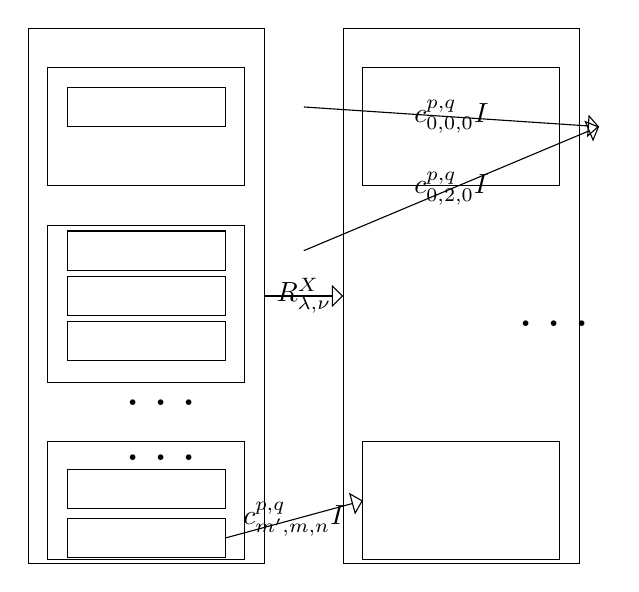
\begin{tikzpicture}
	\draw[color=black] (-9.0,0.75) rectangle (-6.0,-6.05);%upper
\draw[color=black] (-8.75,0.25) rectangle (-6.25,-1.25);%right in upper
\draw[color=black] (-8.5,0.0) rectangle (-6.5,-0.5);%in ``right in upper''
\draw[color=black] (-8.75,-1.75) rectangle (-6.25,-3.75);%middle in upper
\draw[color=black] (-8.5,-1.825) rectangle (-6.5,-2.325);%right in ``middle in upper''
\draw[color=black] (-8.5,-2.4) rectangle (-6.5,-2.9);%middle in ``middle in upper''
\draw[color=black] (-8.5,-2.975) rectangle (-6.5,-3.475);%left in ``middle in upper''
\draw[color=black] (-8.75,-4.5) rectangle (-6.25,-6.0);%left in upper
\draw[color=black] (-8.5,-4.85) rectangle (-6.5,-5.35);%right in ``left in upper''
\draw[color=black] (-8.5,-5.475) rectangle (-6.5,-5.975); %left in ``left in upper''

\draw[color=black] (-5.0,0.75) rectangle (-2.0,-6.05);%lower
\draw[color=black] (-4.75,0.25) rectangle (-2.25,-1.25);%right in lower
\draw[color=black] (-4.75,-4.5) rectangle (-2.25,-6.0);%left in lower

\node at (-7.25,-4.0) {\color{black}{\Huge \dots}};
\node at (-7.25,-4.7) {\color{black}{\Huge \dots}};
\node at (-2.25,-3.0) {\color{black}{\Huge \dots}};

%%\node at (-7.0,1.0) {\color{black}{$I(\lambda)$}};
%%\node at (-2.0,1.0) {\color{black}{$J(\nu)$}};

\draw[-open triangle 90] (-6.0,-2.65) to node {$R_{\lambda,\nu}^X$} (-5.0,-2.65);
\draw[-open triangle 90] (-5.5,-0.25) to node {$c^{p,q}_{0,0,0}I$} (-1.75,-0.5);
\draw[-open triangle 90] (-5.5,-2.075) to node {$c^{p,q}_{0,2,0}I$} (-1.75,-0.5);
\draw[-open triangle 90] (-6.5,-5.725) to node {$c^{p,q}_{m',m,n}I$} (-4.75,-5.25);

	\end{tikzpicture}
\end{center}
\end{frame}
\begin{frame}{Idea}
	\begin{itemize}%[<+(1)->]
		\item \ldots
		\item $\implies$ it would help to compute eigenvalues explicitly;
		\item $\mysbo$ are given by integral kernels; 
		\item $\implies$ eigenvalues are given by integrals;
		\item $\implies$ Proposition \ref{prop:int-st-gg}.
	\end{itemize}
\end{frame}
\begin{frame}[allowframebreaks]{References}
	\bibliographystyle{apalike}
	\nocite{Selberg:411367}
	\nocite{warnaar2010sl3}
	\nocite{dotsenko1985four}
	\nocite{tarasov2003selberg}
%%	\nocite{kobayashi2015symmetry}
%%	\nocite{kobayashi2015differential2}
%%	\nocite{kobayashi2016differential1}
%%	\nocite{kobayashi2014classification}
%%	\nocite{kobayashi2013finite}
%%	\nocite{kobayashi2015program}
\bibliography{intdep}
\end{frame}
\end{document}
